
\chapter{ANALYSIS}
\label{Chapter:Analysis}

\section{Security}

Now we examine and compare OnioNS' central protocols against our security assumptions and expected threat model. 


% Tor circuits work, no global attacker, privacy and anonymity achieved, no crypto breaks
% Tor isn't entirely honest, but the majority is honest
% Eve cannot break Tor in response to OnioNS, Eve cannot guess quorum
% The largest set of agreeing nodes in the Quorum is honest

\subsection{Quorum Selection}

The Quorum nodes have greater attack capabilities than any other class of participants in OnioNS. They have active responsibility over the front of the Pagechain and they must receive, flood, and process new Records from hidden service operators. Malicious Quorums may ignore or substitute received Records and or may attempt to mislead Mirrors. In our threat model, we assume that an attacker, Eve, already has control of some fixed number $ f_{E} $ of routers in the Tor network, and that her nodes may maliciously collude. We also assume that Eve does does not have motivation to compromise Tor in response to the presence of OnioNS and that she cannot predict future Quorums. We therefore feel it safe to examine our Quorum protocols and explore the likelihood of attacks within a probabilistic environment.

The Quorum Derivation protocol selects an $ L_{Q} $-sized subset of routers from the set of Quorum Candidates, and rotates this selection every $ \Delta q $ days. The optimal selection of $ L_{Q} $ and $ \Delta q $ is dependent on both security and performance analysis; our security analysis introduces a bound on both $ L_{Q} $ and $ \Delta q $. For the following evaluations, we feel it safe to discard threats that have probabilities at or below $ \frac{1}{2^{128}} \approx 10^{-38.532} $ --- the probability of Eve randomly guessing a 128-bit AES key, a threat that would violate our security assumptions.

Our security analysis assumes that $ L_{Q} $ will be selected from a pool of 5,400 Quorum Candidates --- the number, as of April 2015, of Tor routers with the Fast and Stable flags, whom we assume are all up-to-date Mirrors. Let $ L_{E} $ be the number of Quorum nodes under Eve's control. Then Eve controls the Quorum if the $ L_{E} $ routers become the largest agreeing subset in the Quorum, which can occur if either more than $ \frac{L_{Q} - L_{E}}{2} $ honest Quorum nodes disagree or if $ L_{E} > \frac{L_{Q}}{2} $. Here we examine the second scenario, which can be theoretically modelled.
%The first scenario requires experimental analysis, so . 

Quorum selection is mathematically an $ L_{Q} $-sized random sample taken from an $ N $-sized population without replacement, where the population contains a subset of $ f_{E} $ entities that are considered special. Then the probability that Eve controls $ k $ Tor routers in the Quorum is given by the hypergeometric distribution, whose probability mass function (PMF) is $ \frac{\binom{f_{E}}{k}\binom{N - f_{E}}{L_{Q} - k}}{\binom{N}{L_{Q}}} $. Then the probability that $ L_{E} > \frac{L_{Q}}{2} $ is given by $ \displaystyle\sum_{x=\ceil{\frac{L_{Q}}{2}}}^{L_{Q}} \frac{\binom{f_{E}}{k}\binom{N - f_{E}}{L_{Q} - k}}{\binom{N}{L_{Q}}} $. Odd choices for $ L_{Q} $ prevents the possibility of network disruption when the Quorum is evenly split in terms of the current Page. We examine the probability of Eve's success for increasing amounts of $ f_{E} $ in Figure \ref{chart:quorumMajority}.

\begin{figure}[htbp]
	\centering
	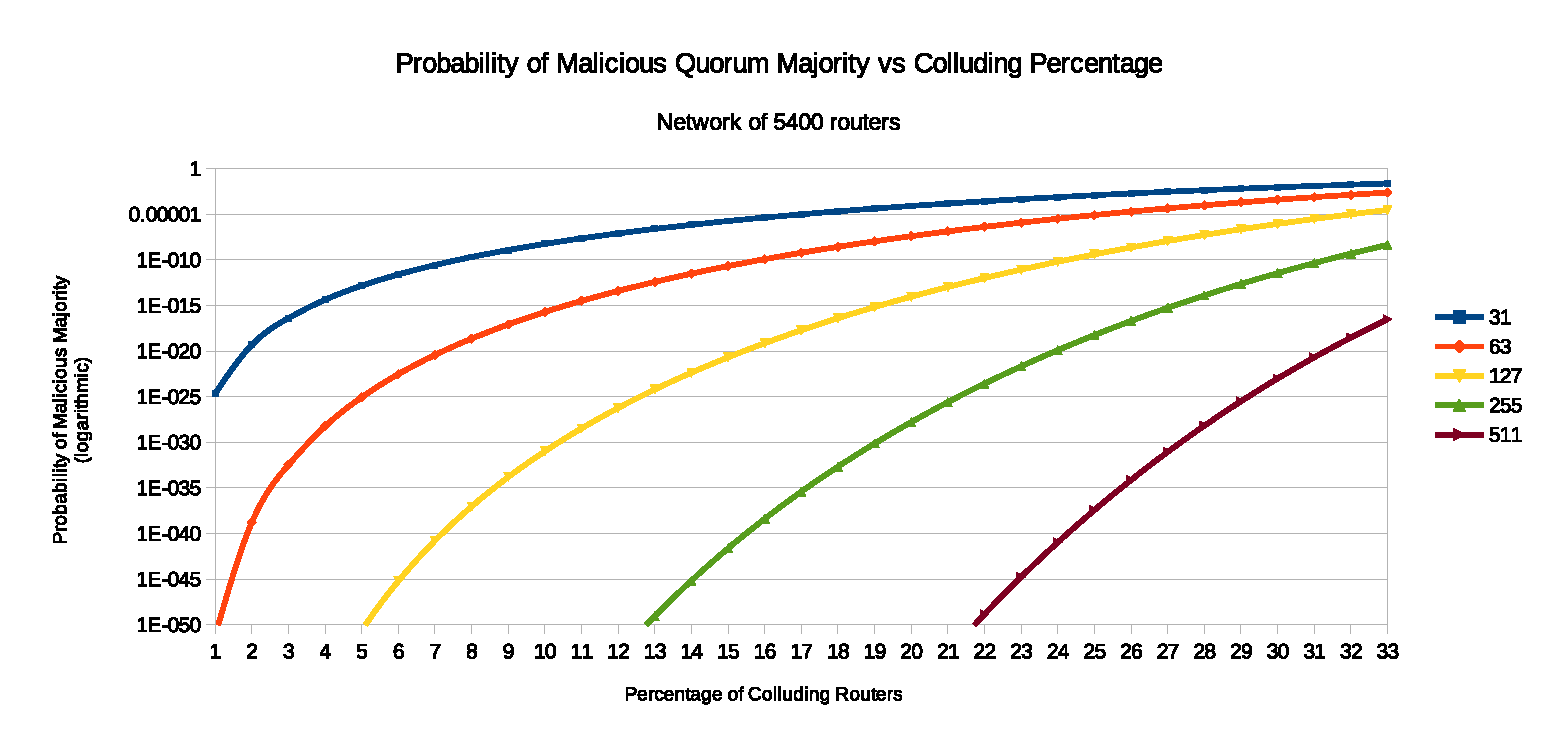
\includegraphics[width=1\textwidth]{analysis/MaliciousQuorumProbability.eps}
	\caption{The probability that Eve controls the majority of the Quorum is given by the PMF of the hypergeometric distribution. We fix $ N $ at 5,400 nodes and graph Eve's success probability as a function of an increasing percentage of Eve-controlled colluding routers. We examine five selections for $ L_{Q} $: 31, 63, 127, 255, and 511. We do not consider percentages beyond 33 percent as 33 percent represents a complete compromise of the Tor network: it is near 100 percent that the three routers selected during circuit construction are under Eve's control, a violation of our security assumptions.}
	\label{chart:quorumMajority}
\end{figure}

Figure \ref{chart:quorumMajority} shows that a choice of $ L_{Q} = 31 $ is suboptimal: the probabilities are above the $ 10^{-38.532} $ threshold for even small levels of collusion. $ L_{Q} = 63 $ likewise fails for percentages above approximately 2, though choices of 127, 255, and 511 fail at levels above approximately 8, 16, and 25 percent, respectively. The figure also suggests that larger Quorums are superior with respect to security. Small Quorums are also less resilient to DDOS attacks at the Quorum in general.

If we assume that Eve controls 10 percent of the Tor network, then we can examine the impact of the longevities of Quorums; over a fixed period of time, slower rotations suggests a lower cumulative chance of selecting any malicious Quorum. If $ w $ is Eve's chance of compromise, then her cumulative chances of compromising any Quorum is given by $ 1 - (1-2)^t $. This gives us a bound estimate on $ \Delta q $. We estimate this over 10 years in Figure \ref{chart:cumulativeProbability}.

\begin{figure}[htbp]
	\centering
	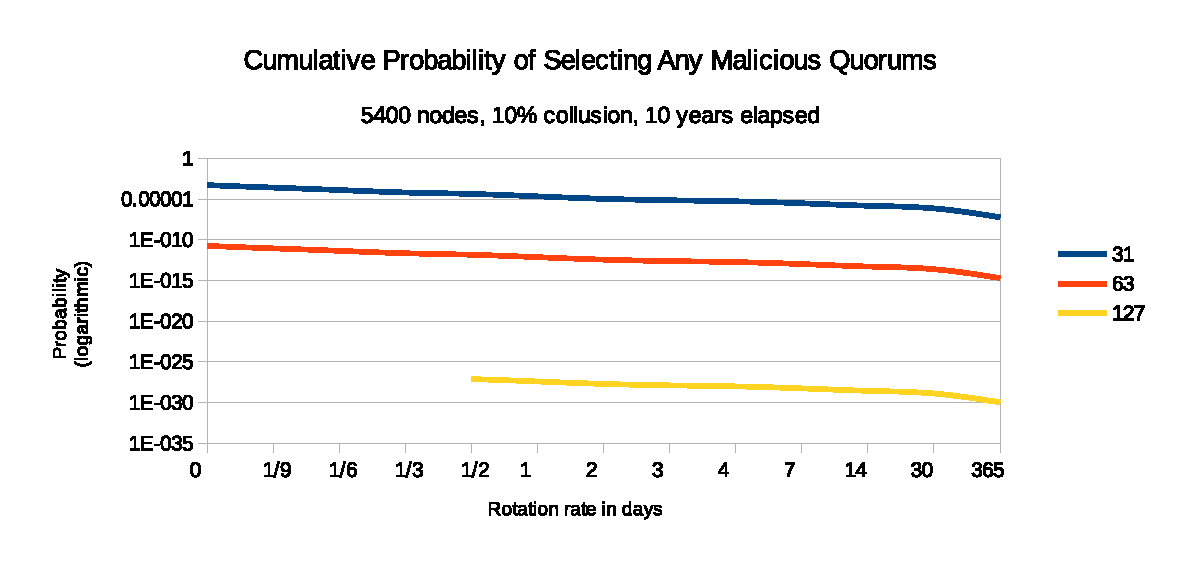
\includegraphics[width=1\textwidth]{analysis/CumulativeMaliciousQuorum.eps}
	\caption{The cumulative probability that Eve controls any Quorum at different rotation rates. We assume 10 percent collusion in a network of 5400 Tor routers, and view across 10 years. We do not graph $ L_{Q} $ values of 255 or 511 as they generate probabilities far below our $ 10^{-38.532} $ threshold; $ L_{Q} = 255 $ and $ L_{Q} = 511 $ produce values less than $ 10^{-58} $ and $ 10^{-134} $, respectively.}
	\label{chart:cumulativeProbability}
\end{figure}

Figure \ref{chart:cumulativeProbability} suggests that while slow rotations (i.e a period of 7 days) generates orders of magnitude less chance than fast rotations, the choice of $ L_{Q} $ is far more significant. Like Figure \ref{chart:quorumMajority}, it also shows that $ L_{Q} = 31 $ and $ L_{Q} = 61 $ are relatively poor choices.

If a selected Quorum is malicious, fast rotation rates will minimize the duration of any disruptions, as shown in Figure \ref{chart:quorumLongevity}. This figure suggests that fast rotations are optimal in that respect, a contradiction to Figure \ref{chart:quorumMajority}. However, given the very low statistical likelihood of selecting a malicious Quorum, we consider this a minor contribution to the decision.

\begin{figure}[htbp]
	\centering
	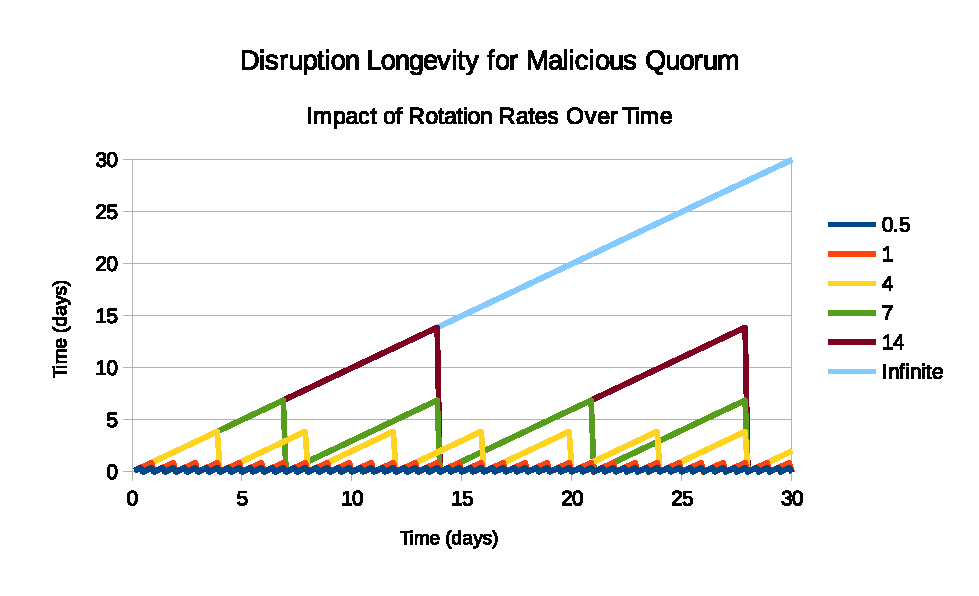
\includegraphics[width=1\textwidth]{analysis/MaliciousLongevityRotations.eps}
	\caption{The duration of malicious Quorums as a function of different rotation rates. Quorums that have very short livetimes (and are thus rotated quickly) minimize the duration of any malicious activity.}
	\label{chart:quorumLongevity}
\end{figure}

Although a malicious Quorum would have the capabilities to deploy a variety of attacks on the network, the proper selections of $ L_{Q} \geq 127 $ and $ \Delta q \geq 1 $ reduces the likelihood of this occurring to near-zero probabilities. We consider this a stronger solution than introducing countermeasures to those attacks. Based on our security analysis, we suggest $ L_{Q} \geq 127 $ and $ \Delta q \geq 1 $. 

\subsection{Entropy of Tor Consensus Documents}

OnioNS can be adapted and deployed on any network that is both fully connected and that contains a common source of entropy. In Tor's case, we use the Tor consensus documents to derive the Quorum, but the consensus documents were designed as a common source of \emph{information}, and thus we must prove that the consensus documents contain enough entropy to be securely used. If there is not enough entropy, Eve can subvert the Quorum Derivation protocol in a variety of attack vectors, including to include her malicious routers in the Quorum, or to reject specific honest routers. As before, we also conclude that ensuring sufficient entropy in these documents is the more effective solution to these threats.

We initialize Mersenne Twister with a 384-bit seed, thus Eve can find $ k $ seeds that generates a desirable scrambled list in $ 2^{192} $ operations on average, or $ 2^{384} $ operations in the worst case. The chance of any of those seeds being selected, and thus Eve successfully carrying out the attack, is thus $ \frac{2^{384}}{k} $.

Eve may attempt to manipulate the consensus document in such a way that the SHA-384 hash is one of these $ k $ seeds. Eve may instruct her Tor nodes to upload a custom status report to the authority nodes in an attempt to maliciously manipulate the contents of the consensus document, but SHA-384's strong preimage resistance and the unknown state and number of Tor nodes outside Eve's control makes this attack infeasible. The time to break preimage resistance of full SHA-384 is still $ 2^{384} $ operations. This also implies that Eve cannot determine in advance the next consensus document, so the new Quorum cannot be predicted. If Eve has compromised at least some of the Tor authority nodes she has significantly more power in manipulating the consensus document for her own purposes, but this attack vector can also break the Tor network as a whole and is thus outside the scope of our analysis. Therefore, the computation required to maliciously generate the quorum puts this attack vector outside the reach of computationally-bound adversaries.

OnionNS and the Tor network as a whole are both susceptible to Sybil attacks, though these attacks are made significantly more challenging by the slow building of trust in the Tor network. Eve may attempt to introduce large numbers of nodes under her control in an attempt to increase her chances of at least one of the becoming members of the Quorum. Sybil attacks are not unknown to Tor, however they are difficulty and slow to carry out in practice as as Tor authority nodes grant consensus weight to new Tor nodes very slowly. The Stable and Fast flags are also granted after weeks of uptime and a history of reliability. As nodes must have these flags to be qualified as a Quorum Candidate, large-scale Sybil attacks are financially demanding and time-consuming to Eve.

Initial results suggest that the Levenshtein distance between consensus documents on consecutive days is large, but that's not the same thing as entropy.

The entropy of the consensus documents can be easily further increased if each of the nine authority nodes contribute a significant amount of random characters into the consensus documents.

\subsection{Outsourcing Record Proof-of-Work}

The Record Generation protocol can safely take place within an offline machine under the operator's control. We designed the protocol to require resigning the Record fields after every round of scrypt so as to require the owner of the private key to also perform the scrypt proof-of-work. Scrypt introduces a cost and its memory demands increases the difficulty of custom hardware and massively-parallel attacks, effectively limiting adversaries to the same hardware as legitimate users. 

However, our protocol does not entirely prevent a hidden service operator from outsourcing the computation to secondary resource. Let Bob be the hidden service and Craig the owner of the computational resource. We assume that Craig does not have Bob's private key. Then,

\begin{enumerate}
	\item Bob creates an initial Record $ R $ and completes the \emph{type}, \emph{nameList}, \emph{contact}, \emph{timestamp}, and \emph{consensusHash} fields.
	\item Bob sends $ R $ to Craig.
	\item Let $ \mathit{central} $ be $\mathit{type} \concat \mathit{nameList} \concat \mathit{contact} \concat \mathit{timestamp} \concat \mathit{consensusHash} \concat \mathit{nonce} $.
	\item Craig generates a random integer $ K $ and then for each iteration $ j $ from 0 to $ K $,
		\begin{enumerate}
			\item Craig increments \emph{nonce}.
			\item Craig sets \emph{PoW} as $ \mathrm{PoW}(\mathit{central}) $.
			\item Craig saves the new $ R $ as $ C_{j} $.
		\end{enumerate}
	\item Craig sends all $ C_{0 \le j \le K} $ to Bob.
	\item For each Record $ C_{0 \le j \le K} $ Bob computes
		\begin{enumerate}
			\item Bob sets \emph{pubHSKey} to his public RSA key.
			\item Bob sets \emph{recordSig} to $ S_{d}(m, r) $ where $ m = \mathit{central} \concat \mathit{pow} $ and $ r $ is Bob's private RSA key.
			\item Bob has found a valid record if $ H(\mathit{central} \concat \mathit{pow} \concat \mathit{recordSig}) \leq 2^{\mathit{difficulty} * \mathit{count}} $
		\end{enumerate}
\end{enumerate}

% todo: calculate chances of Craig computing a correct record

Our protocol ensures that Craig must always compute more scrypt iterations than necessary; Craig cannot generate \emph{recordSig} and thus cannot compute if the hash is below the threshold. Moreover, the scrypt work incurs a cost onto Craig that must be compensated financially by Bob. Thus the Record Generation protocol places a lower bound on the cost paid by Bob.

\subsection{Forgeries and False Negatives Claims}

\emph{What could a Mirror lie about, and what are the implications? I'm really not sure what could happen here because of the Page signatures.}

OnionNS records are self-signed and include the hidden service's public key, so anyone --- particularly the client --- can confirm the authenticity (relative to the authenticity of the public key) and integrity of any record. This does not entirely prevent Sybil attacks, but this is a very hard problem to address in a distributed environment without the confirmation from a central authority. However, the proof-of-work component makes record spoofing a costly endeavour, but it is not impossible to a well-resourced attacker with sufficient access to high-end general-purpose hardware.

Hidden service .onion addresses will continue to have an extremely high chance of being securely unique as long the key-space is sufficiently large to avoid hash collisions.

As we have stated earlier, falsely claiming a negative on the existence of a record is a problem overlooked in other domain name systems. One of the primary challenges with this approach is that the space of possible names so vast that attempting to enumerate and digitally sign all names that are not taken is highly impractical. Without a solution, this weakness can degenerate into a denial-of-service attack if the DNS resolver is malicious towards the client. Our counter-measure is the highly compact hashtable bitset with a Merkle tree for collisions. We set the size of the hashtable such that the number of collisions is statistically very small, allowing an efficient lookup in $ \mathcal{O}(1) $ time on average with minimal data transferred to the client.

\section{Reliability}

%\subsubsection{Flooding}

%\emph{What happens if Quorum nodes are unavailable? How is their unavailability secured for future reference? What are the implications of a Quorum node withholding or forging a Record before flooding their Snapshot out? Can a single node mislead the rest of the Quorum?}

%Although this approach does not entirely thwart Sybil attack, this attack vector is difficulty to impossible to counter in a privacy-enhanced environment, and trading anonymity for defence is highly undesirable.

%\emph{Tor nodes provide no guarantee of availability. What are the implications of Quorum nodes or Mirrors suddenly disappearing? How can data be lost? What if a Quorum node is offline temporarily during active duty, will it catch up?}

%  on Unreliable Hosts

%Tor nodes have no reliability guarantee and may disappear from the network momentarily or permanently at any time. Old \emph{quorums} may disappear from the network without consequence of data loss, as their data is cloned by current \emph{mirrors}. So long as the \emph{quorum} nodes remain up for the $ \Delta i $ days that they are active, the system will suffer no loss of functionality. Nodes that become temporarily unavailable will have out-of-sync \emph{pages} and will have to fetch recent records from other \emph{quorum} nodes in the time of their absence.

\section{Objectives Assessment}

OnioNS achieves all of our original requirements:

\begin{enumerate}
	\item \textbf{The system must support anonymous registrations} --- OnioNS Records do not contain any personal or location information. The PGP key field is optional and may be provided if the hidden service operator wishes to allow others to contact him. However, the operator may be using an email address and a Web of Trust disassociated from his real identity, in which case no identifiable information is exposed.
	\item \textbf{The system must support privacy-enhanced lookups} --- OnioNS performs Domain and Onion Queries through Tor circuits, and under our original assumption that circuits provide strong guarentees of client privacy and anonymity, resolvers cannot sufficiently distinguish users to track their lookups.
	\item \textbf{Clients must be able to authenticate registrations} --- OnioNS Records are self-signed, enabling Tor clients to verify the digital signature on the domain names and check the public key against the server's key during the hidden service protocol. This ensures that the association has not been modified in transit and that the domain name is authentic relative to the authenticity of the destination server.
	\item \textbf{Domain names must be provably or have a near-certain chance of being unique} --- Tor hidden services .onion addresses are cryptographically generated with a key-space of $ 58 ^ {16} \approx 2 ^ {93.727695922} $ and domain names within OnioNS are provably unique by anyone holding a complete copy of the Pagechain.
	\item \textbf{The system must be distributed} --- The responsibilities of OnioNS are spread out across many nodes in the Tor network, decreasing the load and attack potential for any single node. The Pagechain is likewise distributed and locally-checked by all Mirrors, and although its head is managed by the Quorum, these authoritative nodes have temporary lifetimes and are randomly selected. Moreover, Quorum nodes do not answer queries, so they have limited power.
	\item \textbf{The system must be simple and relatively easy to use} --- Domain Queries are automatically resolved and require no input by the user. From the user's perspective, they are taken directly from a meaningful domain name to a hidden service. Users no longer have to use unwieldy .onion addresses or review third-party directories, OnioNS introduces memorability to hidden service domains.
	\item \textbf{The system must be backwards compatible with existing protocols} --- OnioNS does not require any changes to the hidden service protocol and existing .onion addresses remain fully functional. Our only significant change to Tor's infrastructure is the mechanism for distributing hashes for the Quorum Qualification protocol, but our initial technique for using the Contact field minimizes any impact. We also hook into Tor's TLD checks, but this change is very minor. Our reference implementation is provided as a software package separate from Tor per the Unix convention.
\end{enumerate}

Finally, we meet our optional performance objectives:

\begin{enumerate}
	\item \textbf{The system should not require clients to download the entire database} --- Only Mirrors hold the Pagechain, and clients do not need to obtain it themselves to issue a Domain Query. Therefore clients rely on their existing and well-established trust of Tor routers when resolving domain names. However, clients may optionally obtain the Pagechain and post Domain Queries to localhost for greater privacy and security guarantees.
	\item \textbf{The system should not introduce significant burdens to the clients} --- Record verification should occur in sub-second constant time in most environments, and Ed25519 achieves very fast signature confirmation so verifying Page signatures at level 1+ takes trivial time. However, clients also verify the Record's proof-of-work, so for some scrypt parameters the client may spend non-trivial CPU time and RAM usage confirming the one scrypt iteration required to check. We must therefore choose our parameters carefully to reduce this burden especially on low-end hardware.
	\item \textbf{The system should have low latency} --- Domain Queries without any packet delays over Tor low-latency circuits. Its exact performance is largely dependent on circuit speed and the client's verification speed.
\end{enumerate}

We therefore believe that we have squared Zooko's Triangle; OnioNS is distributed, enables hidden service operators to select human-meaningful domain names, and domain names are guaranteed unique by all participants.
